%Falta nombre de los nuevos integrantes...%
\documentclass[10pt,executivepaper]{article}
\usepackage[utf8]{inputenc}
\usepackage[spanish]{babel}
\usepackage{amsmath}
\usepackage{amsfonts}
\usepackage{amssymb}
\usepackage{graphics}
\usepackage{graphicx}
\usepackage[left=2cm,right=2cm,top=2cm,bottom=2cm]{geometry}
\usepackage{imakeidx}
\makeindex[columns=3, title=Alphabetical Index, intoc]
\usepackage{listings}
\usepackage{xcolor}
\usepackage{multicol}
\usepackage{changepage}
\usepackage{float}
\usepackage{cite}
\usepackage{url}
\usepackage{pdfpages}
\usepackage{hyperref}

\definecolor{codegreen}{rgb}{0,0.6,0}
\definecolor{codegray}{rgb}{0.5,0.5,0.5}
\definecolor{codepurple}{rgb}{0.58,0,0.82}
\definecolor{backcolour}{rgb}{0.95,0.95,0.92}

\lstdefinestyle{mystyle}{
    backgroundcolor=\color{backcolour},
    commentstyle=\color{codegreen},
    keywordstyle=\color{magenta},
    numberstyle=\tiny\color{codegray},
    stringstyle=\color{codepurple},
    basicstyle=\ttfamily\footnotesize,
    breakatwhitespace=false,
    breaklines=true,
    captionpos=b,
    keepspaces=true,
    numbers=left,
    numbersep=5pt,
    showspaces=false,
    showstringspaces=false,
    showtabs=false,
    tabsize=3
}

\lstset{style=mystyle}

\title{Compihinador}

\author{}

\date{\today}

\newcommand\tab[1][1cm]{\hspace*{#1}}

\begin{document}
% Portada
%encabezado
\begin{minipage}{0.4\textwidth}
	\begin{flushleft}
		
\includegraphics[scale = 0.05]{imgs/logoescom.png}
	\end{flushleft}
\end{minipage}
\begin{minipage}{0.51\textwidth}
	\begin{flushright}
		
\includegraphics[scale = 0.055]{imgs/logoipn.png}
	\end{flushright}
\end{minipage}
\begin{center}
	\par\vspace{0.5cm}{
		\huge\textbf{Instituto Politécnico Nacional \\*[0.20cm] Escuela Superior de Cómputo}
	}
	\par\vspace{1cm}{
    \huge\textbf{Avance de Proyecto\\*[0.25cm]Compihinador}\\
     \vspace{0.25cm}
		\large\textit{
		%Aquí van sus nombres%
		{Ingeniería de software\\Profesora: Martha Rosa Cordero Lopez\\Grupo: 3CM3\\Integrantes:\\Adrian González Pardo \\Melani Betsabee Valdez Esquivel \\Ángel Edmundo Hernández Rivera \\Mayer Abraham Pérez González\\Semestre: 20/02}}
	}
	\par\vspace{1cm}{
		
\includegraphics[scale=0.5]{imgs/compiladorPortada.jpg}
	}
\end{center}

% Indice
\clearpage
\tableofcontents
\clearpage
%Contenidos
\section{Introducción}
El nombre para el proyecto sera: Compihinador.
\subsection{Objetivo}
El aprendizaje de lenguajes de programación actualmente tiene muchas vertientes en las cuales se puede partir desde lenguajes con una curva de aprendizaje muy sencilla y fluida, hasta lenguajes en los que su curva de aprendizaje implican el uso de algunas notaciones matemáticas o algunas notaciones que impliquen una alta abstracción del lenguaje.
\begin{center}
  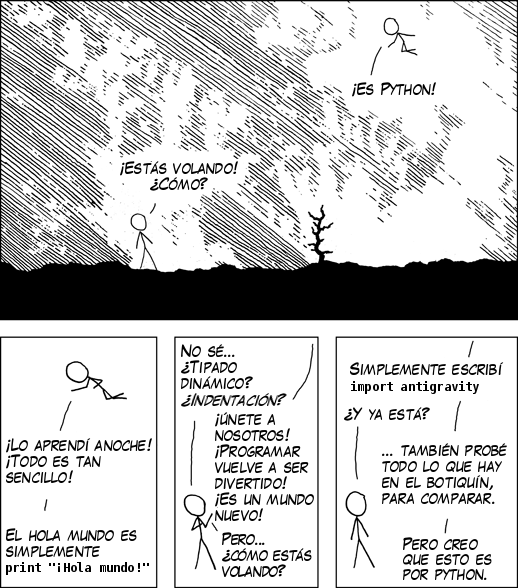
\includegraphics[scale=0.7]{imgs/python.png}
  \\\textit{Figura 1: Python siendo mayormente usado como lenguaje de programación, siendo un lenguaje mayormente interpretado}\\
\end{center}
En algunos casos el uso de lenguajes que son interpretados, generan un consumo significativo de energía y esto en volumenes enormes de información genera problemas en la industria e incluso en las pruebas de performance.
\begin{center}
  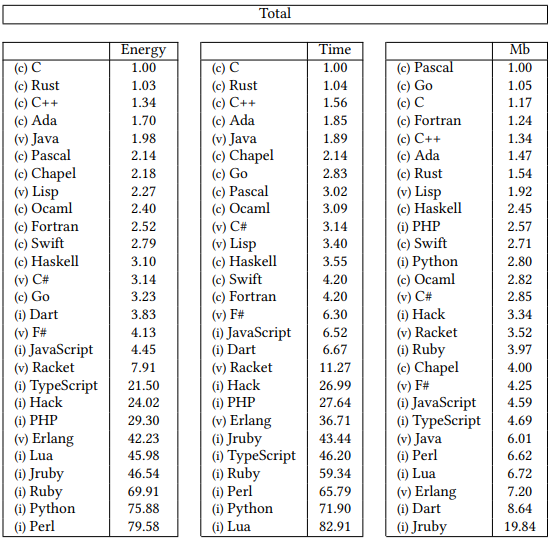
\includegraphics[scale=0.7]{imgs/tabla2.png}
  \\\textit{Figura 2: Tabla de resultados de uso de energía, tiempo y peso en disco de cada lenguaje de programación a los que se realizaron pruebas }\\{\scriptsize Documento de: How Do Energy, Time, and Memory Relate?}
\end{center}
Con base a los datos mostrados en la tabla anterior, se tiene una idea de la diferencia que existe en el consumo de energía, tiempo y memoria al usar un determinado lenguaje de programación. Lo que se contempla para este proyecto es tomar como referentes estos datos para realizar una optimización en cada uno de los parámetros establecidos en la tabla, por lo tanto, se planea que al ejecutar el compilador se puedan obtener valores de costo de energía, tiempo y memoria menores en el uso de un determinado lenguaje de programación con referencia a los que se indican anteriormente.
\subsection{Descripción del Proyecto}
El compilador realizara uso de módulos de herramientas que nos puede proporcionar el software especializado para la creación y descripción de compiladores, en los cuales se buscara realizar una aproximación de que el compilador y el uso de memoria no cree un consumo excedente de energía, memoria o tiempo al generar el código objeto.
\subsection{Funciones Principales}
El compilador es realizado con el fin de poder tener una mejor cercanía con usuarios principiantes los cuales tiene noción de algunos lenguajes de programación como son $Python$, $Ruby$, $Perl$, $etc$.\\Si bien estos lenguajes son considerados lenguajes de alto nivel, se pretende realizar un compilador que realice algunas  operaciones en las que puedan tener un acercamiento a estos tipos de lenguajes y que más tarde puedan mudar de un lenguaje a otro.\\Algunas de las funciones que se consideran son:
\begin{itemize}
    \item Apoyar el aprendizaje del usuario de algún determinado lenguaje de programación.
    \item Capacidad de compilar codigos escritos en diferentes lenguajes de programación. 
    \item Optimización de recursos. (Energía, tiempo y memoria)
\end{itemize}
\subsection{Justificación}
Entender mejor el funcionamiento de los compiladores y su comportamiento a un bajo nivel para poder optimizar y gestionar mejor los recursos a la hora de desarrollar un software de aplicación.
\subsection{Herramientas}
El proyecto a desarrollar contiene algunos puntos a resaltar de los cuales son Hardware y Software en el que se realizara el desarrollo del producto y de su documentación.
\subsubsection{Hardware}
\begin{itemize}
  \item El hardware en el que sera desarrollado el proyecto trabajara bajo una arquitectura x86\_64, debido a que es el actual estándar de desarrollo.
  \item El equipo deseablemente contara con al menos 4GB de RAM.
  \item Procesador dualcore o más cores superior a 1GHz.
\end{itemize}
\subsubsection{Software}
\begin{itemize}
  \item El producto pretende crear un pseudolenguaje que se compila y pretende tener una mejor cercanía con el programador principiante.
  \item El Sistema Operativo en el que se desarrollara y sera la plataforma en la que se ejecutara el proyecto sera en sistema Linux, debido a que las herramientas de trabajo como el analizador léxico, sintactico y semantico pueden encontrarse en paqueterias libres que proporciona Linux.
  \item Se pretende hacer uso de herramientas que proporciona la terminal como el uso de alias y simbolic links para que las llamadas del compilador sean más sencillas en su uso.
  \item Tambien se en la instalación de la paqueteria del compilador se añadiran los manuales pertinentes para que el usuario pueda trabajar correctamente con el producto.
\end{itemize}

\subsection{Innovación}
La innovación del producto de software es el hacer uso de estandares que nos pueden proporcionar el estandar de POSIX, y algunas otras buenas practicas de la programación de modulos de software.\\
Por otro lado tambien es necesario el hacer uso de algoritmos que permitan optimizar el uso de energía que genera la creación y ejecución de código en su entorno de programación.\\
Por lo tanto, si bien es un tiempo corto para la realización de todas las actualizaciones y desarrollo, es bueno planificar el hecho de que pueda existir una aproximación a prototipos del compilador.
\subsection{Complejidad}
De acuerdo a la idea de proyecto a realizar es una tarea larga ya que requiere no solo de uso de herramientas que puede ofrecer el proyecto de GNU/Linux sino que también implica el aprendizaje de las mismas y por otro lado también implica el uso de herramientas que permitan realizar pruebas de estrés y testing como puede realizarlo algunas herramientas de scripting como lo son $Bash$, $sh$, $Ruby$, $Python$.
\subsection{Paradigma de Desarrollo}
El paradigma a utilizar para el proyecto sera el uso de prototipos, así como en la escritura de código sera en el paradigma Estructurado ya que este nos permitirá trabajar con las herramientas que nos ofrece el Sistema Operativo, y un poco de paradigma Orientado a Objetos para hacer uso de algunas herramientas que nos ofrece el mismo, como la modularidad y el uso de algunos empaquetamientos. Nos facilitara la detección de errores o $bugs$ en el proyecto durante su desarrollo.
\begin{center}
  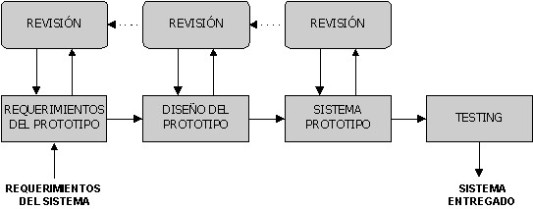
\includegraphics[scale=0.7]{imgs/esq_prototipo.jpg}
  \\\textit{Figura 3: Esquema de "Modelo de Prototipos" }
\end{center}
\subsection{Técnicas de Desarrollo}
Para la recolección de requisitos se llevara acabo una encuesta en la cual nos permitirá recabar información, en la cual podremos interpretar la dirección final y los detalles a pulir del proyecto, en los cuales podremos saber si los encuestados tienen una facilidad o dificultad a la hora de trabajar con un lenguaje de programación compilado.\\
Los hitos planificados del proyecto es trabajarlo con base en el modelo de prototipos para después poder refinar los hitos consiguientes, debido a que es un modelo más sencillos para la realización del producto.\\
También se planea el uso de paradigmas como el orientado a objetos y el estructurado para el desarrollo de los módulos/prototipos.
\subsubsection{Anexo de Prototipo Encuesta 1:}
\begin{enumerate}
    \item ¿Consideras que es muy difícil el escribir un programa en algún lenguaje de programación?
    \item ¿Consideras importante el costo de energía cuando ejecutas un programa?
    \item Bajo tu experiencia. ¿Te interesaría que el compilador que estés manejando sea óptimo en tiempo y en uso de recursos de memoria?
    \item En lo personal. ¿Prefieres que el compilador que estés utilizando sea el mas óptimo en recursos o prefieres que el tiempo de compilación sea menor?
    \item ¿Te agradaría utilizar un compilador bajo la ideología del software libre así como el obtener acceso a su código fuente para mejorar, como un proyecto bajo el estilo de GNU?
    %En la pregunta anterior si es lenguaje? o es compilador?%
    \item ¿Te agradaría la integración de un compilador ligero que permita tener actualizaciones gratuitas como las que se ven disponibles en los repositorios de distribuciones Linux?
\end{enumerate}
\section{Métricas y estimación}
\subsection{Tabla KLDC y Function Point}
\begin{tabular}{|p{3cm}|p{2cm}|p{2cm}|p{2cm}|p{2cm}|}
\hline
Parámetro de & & Complejidad & & \\
medición & Simple & Media & Compleja & Total \\\hline
Número de entradas 3 & 3 & 3 & 3 & 27\\\hline
Número de salidas 2 & 2 & 3 & 3 & 16 \\\hline
Número de archivos 12 & 4 & 4 & 5 & 156 \\\hline
Número de interfaces externas 3 & 3 & 4 & 4 & 33\\\hline
- & - & - & Total & 232 \\\hline
\end{tabular}
\vspace{0.5cm}\\
De acuerdo a las 14 preguntas que se realizan en este método obtenemos la suma de $\Sigma{fi}=63$ por lo que obtendremos el valor de Point Function $PF$ igual a $PF=232*[0.65+0.01*\Sigma{fi}=296$.\\
Ahora con los datos de otra tabla.\vspace{0.5cm}\\
\begin{tabular}{|p{1.83cm}|p{1.83cm}|p{1.83cm}|p{1.83cm}|p{1.83cm}|p{1.83cm}|}
    \hline
    Costo & Personas & Meses & Pag. Doc. & Errores & Esfuerzo \\\hline
    2899 & 4 & 3 & 15000 & 9 & - \\\hline
\end{tabular}
\vspace{0.5cm}\\
De los cuales podemos obtener los siguientes datos
\begin{itemize}
    \item Costo = 9.7622 por función
    \item Calidad = 0.00026
    \item Productividad = 74.24 funciones por persona
    \item Documentación = 50.56 paginas por función
\end{itemize}
\vspace{0.5cm}
Para el caso de KLDC, tomando un KLDC aproximado de 800K :\vspace{0.5cm}
\begin{itemize}
    \item Costo = 0.014445
    \item Calidad = 0.00002
    \item Productividad = 50000
    \item Esfuerzo = 12
\end{itemize}
\vspace{0.5cm}
Si bien podemos notar que este tipo de análisis nos arroja datos que son importantes en la toma de decisiones y adecuaciones del proyecto el planteamiento y la misión de la realización del producto de software se planea no solo para su trabajo a nivel académico, sino que de igual forma podamos lanzar el producto para que la amplia comunidad de software libre pueda ser participe del trabajo.
\subsection{Estimación con COCOMO}
Si bien existen algunos métodos para hacer estimación de un software como por ejemplo el modelo de Putnam Myers, el más utilizado es el propuesto por Barry Boehm, llamado COCOMO o Modelo Constructivo de Costos.\\
Este modelo se divide en tres submodelos: básico, intermedio y avanzado.
\begin{itemize}
    \item El COCOMO básico calcula el esfuerzo y costo del software en función del tamaño del programa expresado en lineas de código.
    \item El COCOMO intermedio calcula el esfuerzo del desarrollo de software en función del tamaño del programa y de un conjunto de conductores de coste que incluye la evaluación subjetiva del producto hardware, personal y de los atributos del proyecto.
    \item El COCOMO avanzado incorpora todas las características de la versión intermedia pero además lleva acabo una evaluación de los impactos de coste en cada etapa (análisis, diseño, etc).
\end{itemize}
De igual manera el COCOMO básico e intermedio tienen en consideración tres modos de desarrollo: orgánico, semi-acoplado y empotrado.
\begin{itemize}
    \item En el Modo Orgánico hablamos de proyectos pequeños en el que trabajas con equipos reducidos con experiencia en la aplicación sobre un conjunto de requisitos poco rígidos.
    \item El Modo Semi-acoplado es para proyectos de software intermedios en tamaño y complejidad, variados niveles de experiencia que deben satisfacer requisitos poco o medio rígidos.
    \item El Modo Empotrado se utiliza para proyectos de software avanzados desarrollados en un conjuntos de hardware, software y restricciones operativos muy fuertes.
\end{itemize}
A continuación se presentan las tablas de valores y ecuaciones para hacer la estimación con el modelo de COCOMO.\\
Tabla de valores para COCOMO básico:
\begin{center}
\begin{tabular}{|p{3cm}|p{1cm}|p{1cm}|p{1cm}|p{1cm}|}\hline
     Proyecto de SW & ab & bb & cb & db\\\hline
     Orgánico & 2.4 & 1.05 & 2.5 & 0.36 \\\hline
     Semi-acoplado & 3.0 & 1.12 & 2.5 & 0.35 \\\hline
     Empotrado & 3.6 & 1.20 & 2.5 & 0.35 \\\hline
\end{tabular}
\end{center}
Ecuaciones para calcular estimación para COCOMO básico:
\begin{center}
    Esfuerzo = E = $abKLDC^{bb}$\\
    Duración = D = $cbE^{bb}$\\
\end{center}
Tabla de valores para COCOMO Intermedio:
\begin{center}
\begin{tabular}{|p{3cm}|p{1cm}|p{1cm}|}\hline
     Proyecto de SW & ai & bi\\\hline
     Orgánico & 3.2 & 1.05 \\\hline
     Semi-acoplado & 3.0 & 1.12 \\\hline
     Empotrado & 2.8 & 1.20 \\\hline
\end{tabular}    
\end{center}
Ecuación para calcular estimación para COCOMO Intermedio:
\begin{center}
    Esfuerzo  = E = $aiKLDC^{bi}XFAE$
\end{center}
Ahora que se ha planteado el Modelo de estimación COCOMO, para nuestro proyecto se ha decidido colocar dentro del submodelo básico en modo semi-acoplado con un número de KLDC aproximado a 800. Por lo que los cálculos para el proyecto son:\\
\begin{center}
    Esfuerzo = $3.0(800)^{1.12}$ = 5352\\
    Duración = $2.5(5352)^{1.12}$ = 37.486
\end{center}
\section{Riesgos}
En la siguiente tabla podemos observar los riesgos a los que el proyecto esta expuesto, con la probabilidad de que sucedan y el impacto que tendrán que son desde algo sencillo hasta algo critico y de igual forma tenemos las estrategias a tomar para solucionar estos riesgos.
\subsection{Tabla de Riesgos}
\begin{center}
    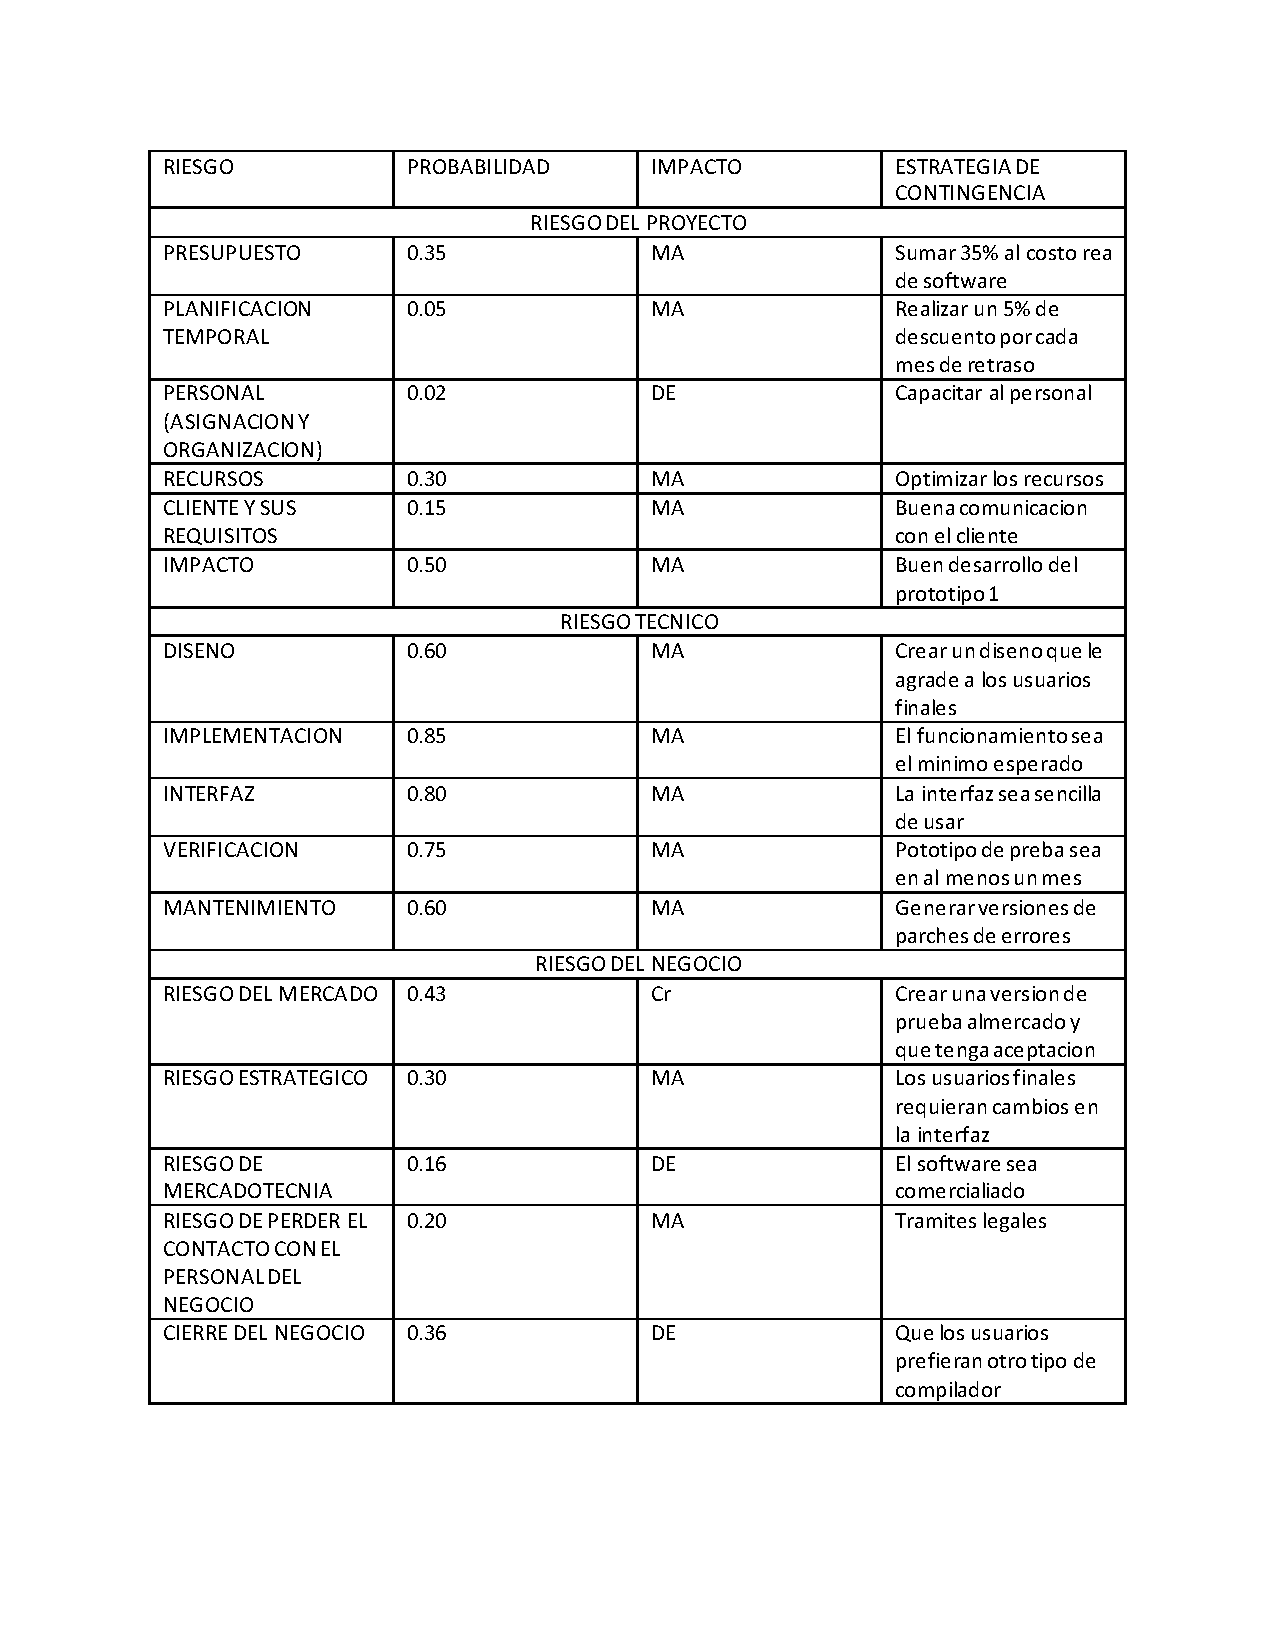
\includegraphics[scale=0.75]{sources/Riesgos.pdf}
\end{center}
\section{Agenda}
\subsection{Cronograma}
En el cronograma veremos las actividades a realizar durante 19 semanas aproximadamente, iniciando en la tercera semana de Enero y concluyendo en tercera semana de Mayo, específicamente el día 22 de Mayo de 2020, día en el cual sera expuesto el proyecto en $ExpoEscom$.
\begin{flushright}
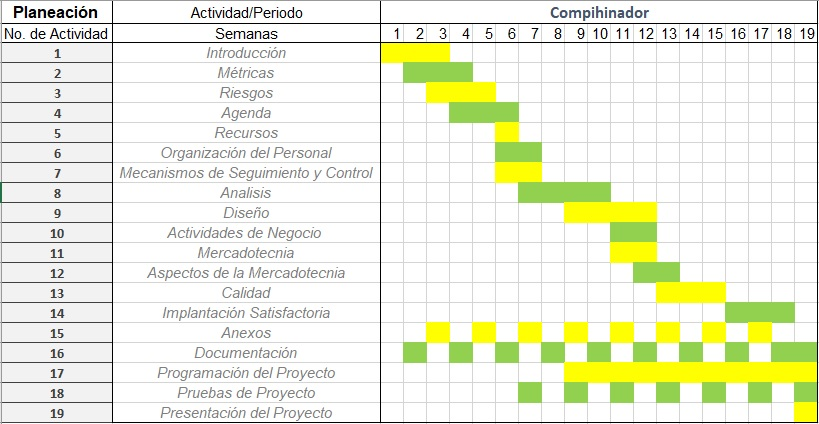
\includegraphics[scale=0.7]{imgs/Cronograma.jpg}
\end{flushright}
\subsection{Gráfica de Gantt}
En la gráfica de Gantt designaremos a los responsables de cada actividad mencionada anteriormente, con una fecha de inicio y una fecha de termino, en algunos casos se presentara mas de 1 responsable, en el caso de que la actividad no pueda ser finalizada en el tiempo establecido, esta tomara la prioridad de todos los integrantes para ser terminada de la manera mas rápida.
\begin{flushright}
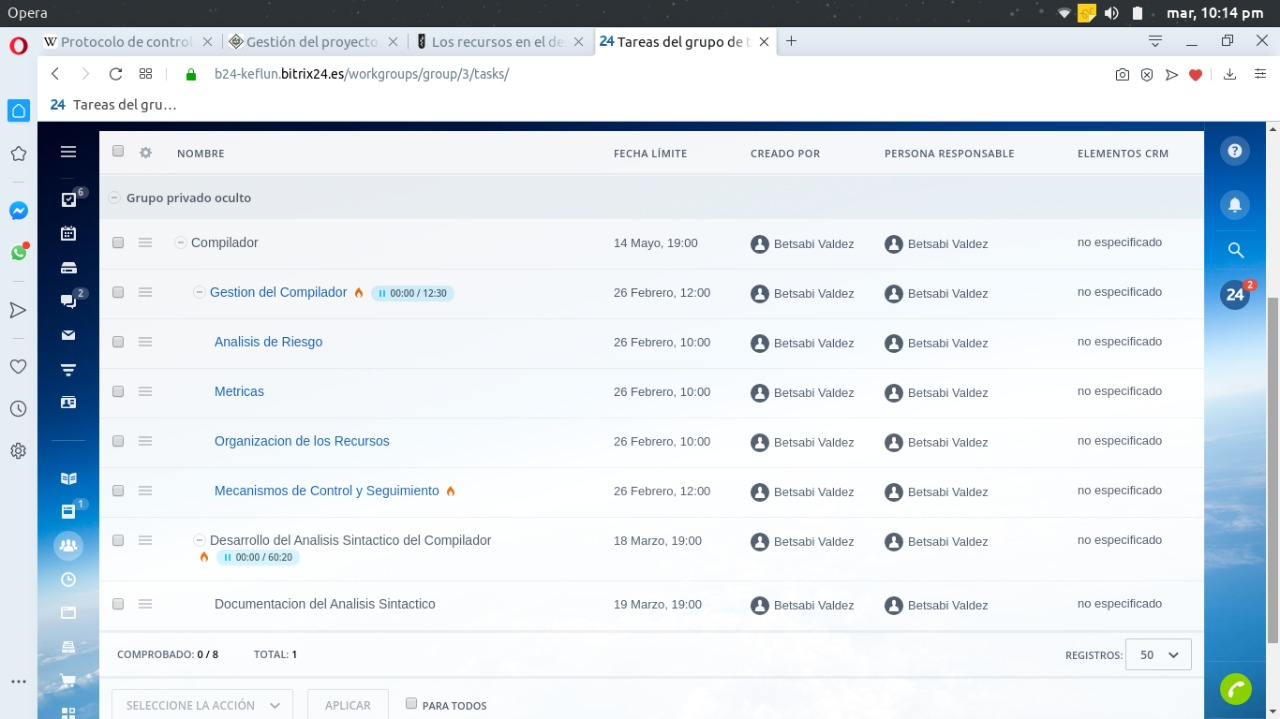
\includegraphics[scale=0.3]{imgs/anexoGantt.jpeg}
\end{flushright}

\section{Recursos}
A continuación se especificaran los recursos que utilizaremos durante la elaboración, desarrollo y programación del proyecto, así como en la documentación de este.
\subsection{Descripción}
\subsubsection{Hardware}
Los equipos varían un poco respecto a sus características y capacidades, pero cumplen con lo esencial para poder desarrollar el proyecto en cada uno de sus sentidos.

\begin{tabular}{|p{3cm}|p{3cm}|p{3cm}|p{3cm}|}
\hline
Modelo & Procesador & RAM & Sistema Operativo  \\\hline
Thinkpad & Core i3 1GHz & 4 GB & Linux  \\\hline
HP 14 Notebook & AMD E1-2100 1GHz & 4 GB & Windows  \\\hline
Lenovo & Core i5 2.49 GHz & 8 GB & Linux  \\\hline
Dell Inspiron 3000 & Core i3 2.4 GHz & 8 GB & Windows  \\\hline
\end{tabular}

\subsubsection{Software}
\begin{tabular}{|p{2.5cm}|p{2.5cm}|p{2.5cm}|p{2.5cm}|p{2.5cm}|}
\hline
Nombre & Especificaciones & Usabilidad & Flexibilidad & Seguridad  \\\hline
Software de Sistema & Sistema operativo Linux Ubuntu 18.04 & Fácil de Usar & Modificable por los desarrolladores & Buen nivel de seguridad \\\hline
Software de Sistema & Sistema operativo Windows 10 & Fácil de Usar & Sin modificaciones por el usuario & Mediano nivel de seguridad  \\\hline
Software de Aplicación & Word & Fácil de Usar & Modificaciones por el usuario & Mediano nivel de seguridad  \\\hline
Software de Aplicación & IDE's & Fácil de Usar & Modificaciones por el usuario & Mediano nivel de seguridad  \\\hline
\end{tabular}

\vspace{0.5cm}
\section{Organización del Personal}
Para definir este aspecto del proyecto se tomo en cuenta la organización del personal según Mantei, quien define los siguientes tipos de organización:\\
\\\underline{Centralizado Controlado (CC)}
\begin{itemize}
    \item El jefe de equipo se encarga de la solución de problemas a alto nivel y la coordinación interna del equipo.
    \item La comunicación entre el jefe y los miembros del equipo es vertical.
\end{itemize}
\underline{Centralizado Democrático (CD)}
\begin{itemize}
    \item Hay comunicación vertical a lo largo de la jerarquía de control.
    \item Las decisiones y los enfoques se hacen por consenso.
\end{itemize}
\underline{Descentralizado Controlado (DC)}
\begin{itemize}
    \item Tiene un jefe que coordina tareas específicas y jefes secundarios que tienen responsabilidades sobre subtareas.
    \item La solución de problemas es una actividad del grupo, pero la implementación de soluciones se reparte entre los subgrupos por el jefe de equipo.
    \item La comunicación entre subgrupos e individuos es horizontal.
    \item También hay comunicación vertical a lo largo de la jerarquía de control
\end{itemize}
\underline{Descentralizado Democrático (DD)}
\begin{itemize}
    \item No tiene un jefe permanente. Se nombran coordinadores de tareas a corto plazo y se sustituyen por otros para diferentes tareas.
    \item Las decisiones y los enfoques se hacen por consenso.
    \item La comunicación entre los miembros del equipo es horizontal.
\end{itemize}
\subsection{Descentralizado Democrático (DD)}
Ya que se conocen los tipos de organización del personal para el proyecto se ha decidido tomar el tipo de organización \textbf{descentralizado democrático} porque se planea realizar el proyecto dividiendo la carga de trabajo de forma proporcional manteniendo una comunicación al mismo nivel, es decir, de forma horizontal y que todos los integrantes sean participes de las decisiones y acciones tomadas para la realización del proyecto.
\section{Mecanismos de Seguimiento y Control}
%Falta de aquí%
El proyecto presentado a través del diagrama de planificación es realizado con el fin de que cada miembro del equipo cumpla en tiempo y forma las tareas pendientes a realizar, así como de igual forma, en conjunto de las herramientas de desarrollo a trabajar y algunas adecuaciones que en la marcha serán pulidas e implementadas, entre las cuales esta el uso de herramientas online para la escritura de reportes y de control de versiones de los avances que se estén realizando en el avance del proyecto. Cada tarea sera asignada en especifico a algún miembro del equipo con un tiempo definido para ser realizada.

\section{Anexos}
%Falta aqui%
En esta sección se encuentran todos los enlaces y referencias que se utilizo para la realización del proyecto.
\subsection{Encuesta}
Encuesta aplicada a usuarios. \href{https://forms.gle/8S5iEbKtkk9fVoKZ8}{{\underline{Enlace aquí}}}
\begin{center}
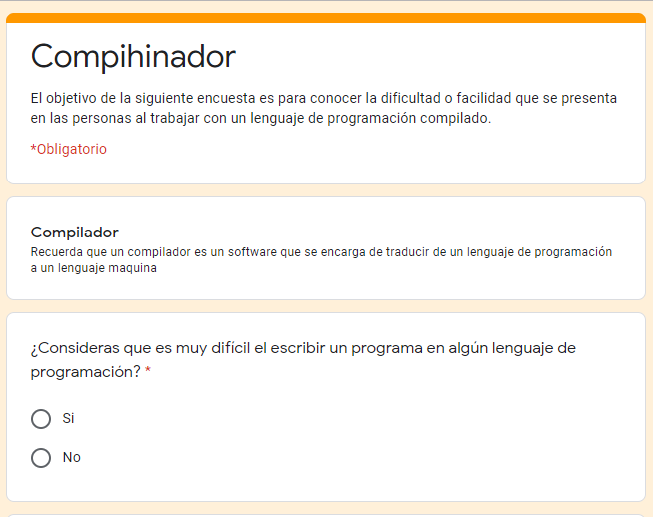
\includegraphics[scale=0.5]{imgs/Encuesta1.png}
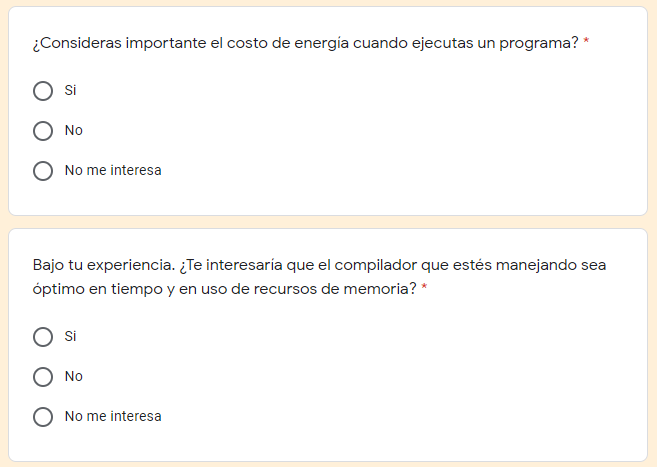
\includegraphics[scale=0.5]{imgs/Encuesta2.png}
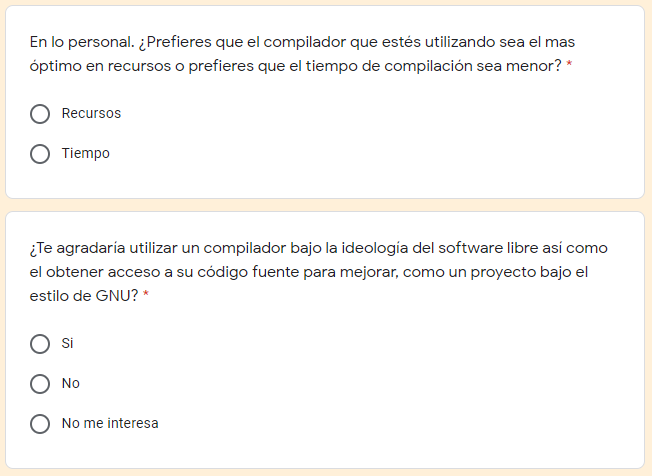
\includegraphics[scale=0.5]{imgs/Encuesta3.png}
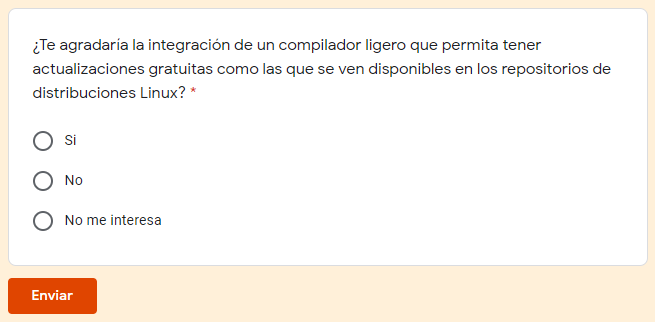
\includegraphics[scale=0.5]{imgs/Encuesta4.png}
\\\textit{Figuras 5,6,7 y 8: Encuesta aplicada a usuarios acerca del proyecto }\\
\end{center}
\subsection{Tabla de Lenguajes}
Tabla de lenguajes en uso de energía y recursos, obtenido de: 
\href{https://greenlab.di.uminho.pt/wp-content/uploads/2017/10/sleFinal.pdf}{{\underline{Enlace aquí}}} o escanea:\\
\begin{center}
\includegraphics[scale=0.75]{imgs/qrAnexo1.png}\end{center}
\printindex

\end{document}
